\documentclass[tikz,border=2pt,11pt]{standalone}
\usetikzlibrary{calc}
\usetikzlibrary{arrows.meta}
\usetikzlibrary{positioning}
\usetikzlibrary{decorations.pathreplacing}
\usepackage{amsmath}
\usepackage{amssymb}
\usepackage{graphicx}
\usepackage{xcolor}
\usepackage{tikz}
\newcommand{\F}{\mathbb{F}}
\newcommand{\N}{\mathbb{N}}
\newcommand{\Z}{\mathbb{Z}}
\newcommand{\WL}{\mathrm{WL}}
\newcommand{\AC}{\mathrm{AC}}
\begin{document}
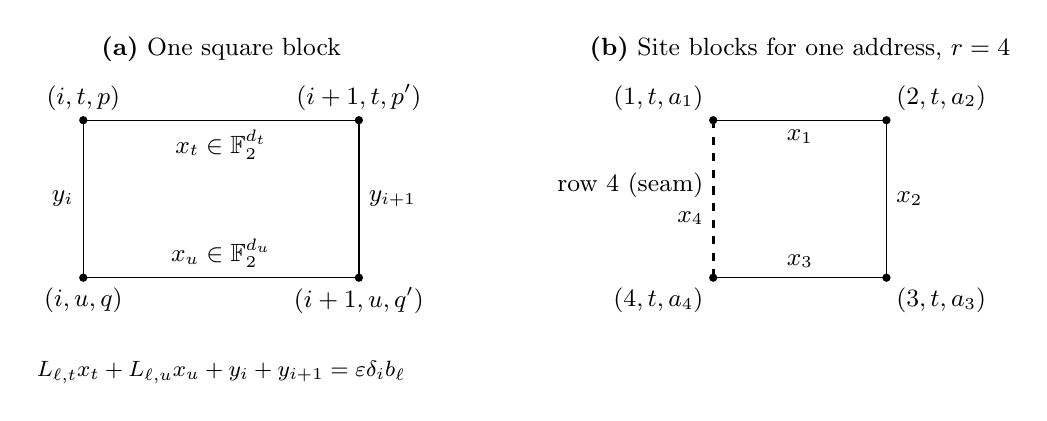
\begin{tikzpicture}[font=\small,line width=0.5pt]
  \node at (1.75,0.9) {\textbf{(a)} One square block};
  \draw (0,0) -- (3.5,0) -- (3.5,-2) -- (0,-2) -- cycle;
  \fill (0,0) circle (1.5pt);
  \fill (3.5,0) circle (1.5pt);
  \fill (3.5,-2) circle (1.5pt);
  \fill (0,-2) circle (1.5pt);
  \node[above] at (0,0) {$(i,t,p)$};
  \node[above] at (3.5,0) {$(i+1,t,p')$};
  \node[below] at (0,-2) {$(i,u,q)$};
  \node[below] at (3.5,-2) {$(i+1,u,q')$};
  \node[below] at (1.75,0) {$x_t\in\F_2^{d_t}$};
  \node[above] at (1.75,-2) {$x_u\in\F_2^{d_u}$};
  \node[left] at (0,-1) {$y_i$};
  \node[right] at (3.5,-1) {$y_{i+1}$};
  \node[font=\footnotesize] at (1.75,-3.2)
    {$L_{\ell,t}x_t+L_{\ell,u}x_u+y_i+y_{i+1}
       =\varepsilon\delta_i b_\ell$};

  \node at (9.1,0.9) {\textbf{(b)} Site blocks for one address, $r=4$};
  \draw (8,0) -- (10.2,0) -- (10.2,-2) -- (8,-2);
  \draw[dashed,very thick] (8,-2) -- (8,0);
  \fill (8,0) circle (1.5pt);
  \fill (10.2,0) circle (1.5pt);
  \fill (10.2,-2) circle (1.5pt);
  \fill (8,-2) circle (1.5pt);
  \node[above left] at (8,0) {$(1,t,a_1)$};
  \node[above right] at (10.2,0) {$(2,t,a_2)$};
  \node[below right] at (10.2,-2) {$(3,t,a_3)$};
  \node[below left] at (8,-2) {$(4,t,a_4)$};
  \node[below] at (9.1,0) {$x_1$};
  \node[right] at (10.2,-1) {$x_2$};
  \node[above] at (9.1,-2) {$x_3$};
  \node[left,align=right] at (8,-1) {row $4$ (seam)\\$x_4$};
\end{tikzpicture}
\end{document}
